\section{Extension du support exécutif}\label{sec:openmp:runtime}

\cite{Virouleau2016b}, Using data dependencies to improve task-based scheduling strategies on numa architectures

\subsection{Hiérarchiser le support exécutif}

ici on parle de la vision hiérarchique de la machine


\subsection{Heuristiques basé sur la localité des données}\label{sec:contrib:ws:heuristics}

GRAPHE : 5.4.2, schéma step-by-step des heuristiques envisagées ?

\subsection{Distribution of ready tasks : WSpush strategies}

This section describes four different ways of pushing ready tasks to a NUMA system places.
Two of them are data-oblivious while the other two rely on the dependencies expressed using the \verb!depend! keyword on OpenMP tasks.

The \verb/pLoc/ strategy makes a processor push ready tasks to
    its own place, while the \verb/pLocNum/ strategy makes a processor push ready tasks to the place of its NUMA node (\emph{local NUMA node}).
The \verb/pNumaW/ strategy pushes tasks on the node-level place corresponding to the NUMA node where most of their output data are allocated to (W stands for Write).
The last WSpush strategy, called \verb/pNumaWLoc/, behaves almost the same than \verb!pNumaW! except that if
    the data are allocated to the NUMA node of the processor pushing the task, we directly push the task to this processor's place instead of pushing it to the node-level place (Loc stands for Local).
    
It's important to note that \verb!pLoc! and \verb!pLocNum! does not take initial data placement into account, while \verb!pNumaW! and \verb!pNumaWLoc! are both aware of where a task's data are physically allocated and which of them are written, thanks to the OpenMP \verb!depend! keyword.

\subsection{Dynamic load balancing using work-stealing : WSselect strategies}
\label{sec:ws_select}

Another important step when implementing work-stealing is the selection of the victim processor we want to steal from.
This section describes the selection strategies we implemented, that take the architecture memory hierarchy into account.
The first two strategies, \verb!sRand! and \verb!sRandNuma! are similar to those studied in~\cite{DBLP:journals/ijhpca/OlivierPWSP12}
and distinguish two levels of hierarchy : the processor level and the NUMA node level.
\verb/sRand/ selects a random processor's place while \verb/sRandNuma/ selects a random NUMA node's place.
We additionally implemented several strategies mixing both levels of hierarchy,
described below.

%\begin{figure}[t]
%  \centering
%  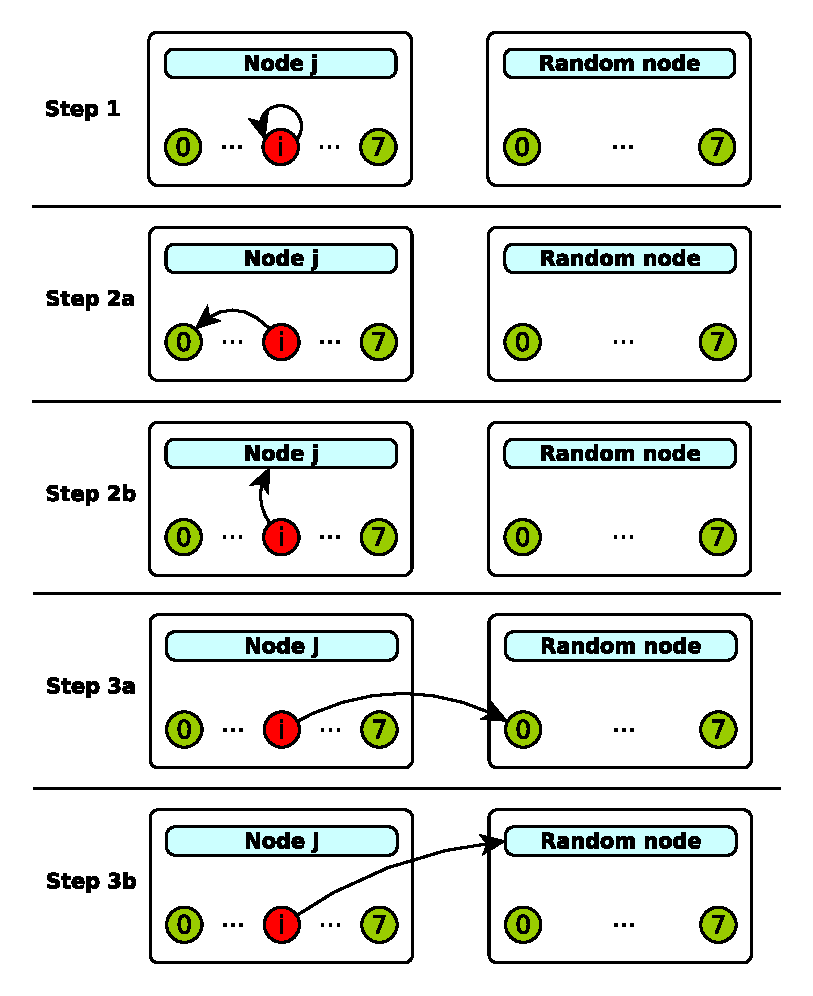
\includegraphics[scale=0.45]{figures/strategies.pdf}
%  \caption{Illustration of the "sProcNuma" strategy}
%\label{fig:detail-strategy}
%\end{figure}
\begin{itemize}
  \item \verb/sProcNuma/ : First, we browse the processor's place. Upon failure, we browse the topology in the following order : we first browse one of the neighbor processors ; when all the neighbors have been visited, we browse the local NUMA place ; we continue by browsing all the processors' places from a random remote node and we eventually consider the place of its NUMA node.
  \item \verb/sNumaProc/ : This strategy is similar, except we always look at the
    NUMA place before looking at the processors' place.
  \item \verb/sProc/ : In this strategy the stealer will visit only the
    processors' places and its own NUMA place.
  \item \verb/sNuma/ : In this strategy the stealer will visit only NUMA places
    and its neighbors. 
\end{itemize}

Like proposed in \cite{Olivier:2012:CMW:2388996.2389085}, all these strategies come in two versions : a \verb!strict! version in which we prevent processors from stealing from other NUMA nodes to improve data locality and a \verb!loose! version where these restrictions do not apply.

\subsection{Distribution of initial ready tasks : WSpush\_init strategies}
\label{sec:ws_push_init}
We refer to \emph{initial tasks} when considering the sources of a task dependency graph, usually declared at the beginning of an OpenMP parallel region.
These tasks are basically the first ones to be marked as ready and to be distributed over the platforms' places.
We have implemented two initial tasks distribution strategies : \verb!cyclicnuma! which distributes the tasks in a round-robin fashion over the NUMA nodes, and \verb!randnuma! which randomly distributes the tasks over the NUMA nodes.
Note that unlike \verb!numactl!, the strategies we implemented consider the whole data appearing in the OpenMP task \verb!depend! clause instead of working at the page level. In other words, while the two memory pages holding an 8K-wide array would be distributed on different nodes by \verb!numactl --interleave=all!, they are always assigned to the same NUMA node when using one of our data distribution strategies.


revoir le titre.

ici on parle du fait qu'on peut faire de l'initialisation selon le souhait du programmeur

\subsection{Détails d'implémentation}

?
